\documentclass[conference,a4paper]{IEEEtran}

\usepackage{cite}
\usepackage{amsmath,amssymb,amsfonts}
\usepackage{algorithmic}
\usepackage{graphicx}
\usepackage{textcomp}
\usepackage{xcolor}
\usepackage{url}
\usepackage{hyperref} % TODO: remove before submission
\usepackage{lipsum}

\begin{document}

\title{Graph-Based Representation of Contour Images: A Step Toward Self-Describing Explainable AI}

\author{
    \IEEEauthorblockN{Mykyta Lapin\IEEEauthorrefmark{1}}
    \IEEEauthorblockA{ORCID: \url{https://orcid.org/0009-0003-6307-1172}}
    \and
    \IEEEauthorblockN{Kostiantyn Bokhan\IEEEauthorrefmark{1}}
    \IEEEauthorblockA{ORCID: \url{https://orcid.org/0000-0003-3375-2527}}
    \and
    \IEEEauthorblockA{\IEEEauthorrefmark{1}National Technical University "Kharkiv Polytechnic Institute", Kharkiv, Ukraine}
}

\maketitle

\begin{abstract}
Opaque perception pipelines hinder trust and diagnosis in real-world AI systems. We present a graph-based representation for contour images that makes structure the carrier of explanations. The approach encodes visual patterns as attributed graphs where nodes represent critical points (endpoints, corners, junctions) and edges represent connecting line segments, with semantic tags and geometric attributes attached directly to graph elements. Crucially, we demonstrate how multiple graph instances of the same class can be reduced to form stable \textit{concept attractors}---canonical graph structures that capture shared topological and parametric patterns while filtering instance-specific variations. This concept formation process operates through iterative structural and parametric reduction without backpropagation, enabling few-shot learning from minimal training data. We validate the approach on MNIST handwritten digits, where concepts formed from 5--6 training samples achieve meaningful classification through graph matching. By encoding semantics explicitly in graph structure rather than in opaque weight matrices, the approach advances explainable AI while maintaining competitive few-shot learning performance.
\end{abstract}

\begin{IEEEkeywords}
explainable AI (XAI), contour images, attributed graphs, self-describing models, structural representation, traceability
\end{IEEEkeywords}

\section{Introduction}

Modern perception systems achieve impressive accuracy yet often operate as opaque pipelines, making it difficult for practitioners to understand \textit{why} a particular decision was reached or \textit{where} evidence resides in the input. Post-hoc explanation techniques can be helpful, but they typically project reasoning onto models that were not designed to be interpretable, yielding artifacts that are hard to validate or reuse across tasks. Modern post-hoc explanation methods such as LIME and SHAP can be adversarially manipulated or yield inconsistent attributions \cite{ribeiro2016should,slack2020foolinglimeshapadversarial,hooshyar2024problems}. Knowledge-graph‐based approaches demonstrate that explicit graph structures improve interpretability over opaque weight matrices \cite{rajabi2024knowledge}. This gap undermines trust, slows diagnosis when things fail, and complicates compliance in domains that require traceable decision paths. To address these problems, we argue for \textbf{human-readable internal structure} as a first-class design goal rather than an afterthought.

Our central idea is to make \textbf{structure the carrier of explanations}. Instead of relying primarily on latent vectors whose semantics are implicit, we encode visual information as \textbf{graphs} whose semantics are explicit. In the context of 2D images, \textbf{contours} provide a compact, model-agnostic description of shape: endpoints, corners, and junctions capture where curves meet or terminate, while \textbf{line segments} capture how they connect. We represent this as a bipartite graph where both critical points and line segments are nodes, with edges denoting spatial adjacency. This design makes line segments first-class queryable entities rather than mere connectivity markers. Crucially, \textbf{attributes and tags} attached to graph elements preserve meaning directly inside the representation: node types encode structural roles, geometric parameters capture orientation and position, and connectivity patterns reveal topological properties. Explanations become navigable objects: cycles justify closed contours, node degree reveals branching structure, and attribute ranges encode acceptable variation.

The goal of this paper is therefore modest and focused: we \textbf{show how contours can be encoded as attributed graphs} that remain readable to both humans and machines, and we demonstrate how multiple graphs of the same class can be reduced to form \textbf{concept attractors}---stable canonical structures suitable for classification. We present the method at a \textbf{high level}, emphasizing what is represented rather than prescribing specific extraction algorithms. Concretely, we: (i) define a minimal vocabulary of node/edge types and attributes; (ii) describe normalization choices that make the representation invariant to scale and translation; and (iii) outline how \textbf{structural reduction rules} iteratively merge training samples into generalized concepts that preserve shared topology while abstracting parametric variation. We validate the approach on MNIST handwritten digits, demonstrating that concepts formed from 5--6 training samples per class enable meaningful few-shot classification through graph matching, with aggregate structural metrics confirming that the representation remains compact and interpretable.

What this paper does \textbf{not} attempt is equally important. We do not propose or benchmark a new contour-extraction algorithm; we assume edges or skeletons are available from any standard method. We do not optimize classification performance or compare against state-of-the-art benchmarks; our goal is to demonstrate the viability of graph-based concept formation and the interpretability it affords. We also avoid deep theory beyond what is necessary to state the representation and its reduction operators. Those aspects---algorithmic optimizations, large-scale benchmarking, and formal convergence properties---are intentionally left for \textbf{follow-up work}, where each topic can be treated with appropriate depth.

\section{Background and Related Work}

\subsection{Limitations of Post-hoc Explainability Methods}

Current approaches to explainable AI (XAI) predominantly rely on post-hoc explanation techniques applied to already-trained models. These methods, exemplified by LIME (Local Interpretable Model-agnostic Explanations) and SHAP (SHapley Additive exPlanations), attempt to reverse-engineer model behavior by approximating decision boundaries locally or assigning feature importances through game-theoretic principles \cite{ribeiro2016should,lundberg2017unified}. 

While these techniques have gained widespread adoption, recent studies have exposed fundamental vulnerabilities. Slack \emph{et al.} \cite{slack2020foolinglimeshapadversarial} demonstrated that both LIME and SHAP can be adversarially manipulated: a biased classifier can be scaffolded to behave discriminatorily on real data while appearing fair on perturbed samples, thus fooling explanation methods into generating innocuous attributions. These attacks exploit the perturbation-based nature of post-hoc methods, revealing that their outputs are unreliable in adversarial settings. Furthermore, both methods suffer from high sensitivity to model choice, feature collinearity, and hyperparameter selection, complicating their interpretation and reuse across tasks \cite{hooshyar2024problems}. The fundamental problem remains that post-hoc explanations are artifacts constructed \textit{after} the model is trained, not integral to its decision-making process, making it difficult to validate or trace explanations back to the input with confidence.

\subsection{Graph-Based Representations in Vision}

Recent advances in computer vision have demonstrated the value of graph-based representations over traditional grid-structured approaches. Vision GNNs (ViG) treat images as graphs where patches serve as nodes and content-based connectivity replaces spatial locality, enabling more flexible and interpretable visual reasoning \cite{han2022vision}. This representation naturally captures irregular and hierarchical object structures that grids struggle to express. 

Beyond patch-based methods, structured shape representations have long been studied in pattern recognition. Contours and skeletons represent complementary views of shape: contours encode boundaries while skeletons capture thickness and topological structure \cite{chatbri2016comparative}. Shen \emph{et al.} \cite{shen2016shape} proposed Skeleton-associated Shape Context (SSC) descriptors that combine contour geometry with skeletal information, demonstrating that fusing these representations improves shape recognition. More generally, attributed graphs where nodes and edges carry semantic and geometric metadata have proven effective for encoding visual patterns in a queryable, human-readable form \cite{wang2023graph}. Knowledge graphs similarly show that explicit graph structures improve interpretability over opaque weight matrices in neural systems \cite{rajabi2024knowledge}.

The key insight motivating the present work is that visual structure itself can be the primary carrier of semantic information, rather than being embedded implicitly in learned weights. If visual patterns are encoded directly as graph attributes and topology, explanations emerge naturally from the representation itself rather than being grafted on post-hoc.

\subsection{Graph Matching and Edit Distance}

Comparing and matching graphs is fundamental to structural pattern recognition. Graph Edit Distance (GED) provides a principled measure of graph dissimilarity, defined as the minimum cost sequence of edit operations (node/edge insertion, deletion, substitution) to transform one graph into another \cite{serratosa2015,lucbrun2023}. GED is NP-hard in the general case, but for moderate-sized graphs and when structure dominates over metric details, tractable approximations suffice.

Recent work has combined deep learning with GED computation. Wang \emph{et al.} \cite{wang2021combinatorial} proposed a hybrid approach that learns node embeddings via GNNs while leveraging dynamic programming to prune the search space, achieving both interpretability and efficiency. Liu \emph{et al.} \cite{liu2023mata} further improved scalability by learning node matchings directly rather than regressing GED, enabling the method to scale to larger graphs while recovering edit paths. Peng \emph{et al.} \cite{peng2021graph} introduced GED-specific loss functions encoding multiple optimal matchings and one-to-one constraints. These developments show that graph matching, when integrated with learning, can be made efficient enough for practical classification tasks while remaining interpretable through explicit path recovery.

\subsection{Few-Shot Learning and Concept Formation}

Few-shot learning addresses the challenge of learning new concepts from minimal labeled data. The field primarily operates within the meta-learning framework, where a learner is exposed to a distribution of \emph{tasks}---each mimicking the few-shot scenario---rather than individual examples. This episodic training teaches the algorithm to generalize across tasks and adapt quickly to novel classes \cite{finn2017model,gharoun2023meta}.

Within meta-learning, several paradigms exist. Metric learning approaches, exemplified by Prototypical Networks, learn an embedding space in which classification is performed via distance to class prototypes (the mean of support examples in embedding space) \cite{snell2017prototypical}. Memory-augmented networks store and retrieve learned experience, while gradient-based methods (e.g., MAML) optimize for fast inner-loop adaptation \cite{finn2017model}. Meta-Transfer Learning extends this by learning to scale and shift pre-trained feature extractors \cite{sun2019meta}, achieving strong few-shot performance on benchmarks like miniImageNet.

The present work differs in that it does not rely on deep feature extractors or gradient-based optimization. Instead, it formulates concept formation through iterative \emph{structural reduction}---successive merging and abstraction of graph instances to form canonical attractors. This approach is closer in spirit to classical clustering and prototype formation but operates directly on graph topology and attributes, requiring no backpropagation.

\subsection{Neuro-Symbolic AI and Structured Reasoning}

An emerging paradigm seeks to bridge neural learning and symbolic reasoning, combining the pattern recognition of neural networks with the logical transparency of symbolic systems. Neuro-symbolic AI systems integrate knowledge graphs, symbolic rules, and explicit reasoning with learned representations, yielding models that are both adaptive and interpretable \cite{nawaz2025review,ismaeil2022towards}. By encoding domain knowledge and relationships as graphs or logical statements, such systems provide introspectable decision paths and the ability to explain conclusions through formal reasoning steps.

Knowledge-graph-based approaches to interpretability have demonstrated that explicit graph structures enable more trustworthy and verifiable reasoning than opaque weight matrices \cite{rajabi2024knowledge}. GNNExplainer \cite{ying2019gnnexplainer} generates subgraph explanations for GNN predictions by maximizing mutual information between predictions and subgraph distributions. These methods show that when structure is explicit and queryable, explanations can be validated and refined without post-hoc approximation.

\subsection{Related Work Summary}

The above background reveals a gap in current practice: while post-hoc XAI methods are widely deployed, they are vulnerable to adversarial manipulation and cannot trace explanations faithfully back to the input. Graph-based vision methods and symbolic reasoning systems offer promise, but few approaches combine explicit structure with minimal training data in a single, self-describing framework. The present paper advances this agenda by showing how contour graphs can encode shape semantics directly, and how multiple such graphs can be reduced to stable concept attractors without gradient-based training. By making structure, not weights, the carrier of explanation, the approach aims to achieve interpretability and few-shot capability in a unified framework.

\section{Graph Representation}

\subsection{Node Types and Bipartite Structure}

The system represents image contours as bipartite graphs alternating between \emph{Point} nodes and \emph{Line} nodes. Crucially, line segments are represented as first-class nodes rather than edges, enabling them to carry attributes such as length, direction, and orientation. Point nodes and Line nodes connect via bidirectional \texttt{CONNECTED\_TO} relationships, creating a traversal pattern of the form Point $\to$ Line $\to$ Point $\to$ Line.

Point nodes are classified into four topological types: \textbf{EndPoint} (terminal nodes of open contours), \textbf{CornerPoint} (nodes marking sharp directional changes, storing an angle attribute), \textbf{IntersectionPoint} (nodes where multiple segments meet), and \textbf{StartPoint} (anchor nodes for graph traversal). Each node in Neo4j carries multiple labels (e.g., \texttt{["Point", "CornerPoint"]}), enabling both type-specific queries and generic structural operations. This bipartite design separates topological structure (points) from geometric properties (line segments), facilitating explicit feature extraction and structural comparison.

\subsection{Attributes and Parameters}

Each node type carries attributes that encode geometric, directional, and topological properties. \textbf{Point nodes} store $(x, y)$ coordinates and their normalized counterparts as well as an angle value between the vectors it connects. \textbf{Line nodes} store endpoint pairs $(x_1, y_1, x_2, y_2)$ and a length attribute (magnitude), enabling direct access to segment geometry without recomputing from connected points.

Directional attributes capture spatial orientation. Each Line node is assigned a \emph{quadrant} (I, II, III, IV) based on the displacement vector from its start point, computed when the coordinate system is translated to that point. Lines also carry \emph{horizontal direction} (LEFT, RIGHT, NONE) and \emph{vertical direction} (TOP, BOTTOM, NONE) labels that encode relative positioning. These attributes, computed by visitor classes during graph traversal, enable comparisons of spatial development patterns across different contours.

\subsection{Normalization}

To achieve scale and translation invariance, all coordinates and distances are normalized. Point coordinates are transformed to a centered system ranging $[-1, 1]$ via the formula $\text{normalized}_x = (x - \text{center}_x) / \text{center}_x$, and similarly for $y$ (see Figure~\ref{fig:coordinate_systems}). This normalization ensures that concept attractors remain stable across variations in image size, position, and aspect ratio, enabling shape recognition independent of viewing conditions.

% TODO: fix the relative coordinate system image to include the axis from -1 to 1
\begin{figure}[!t]
    \centering
    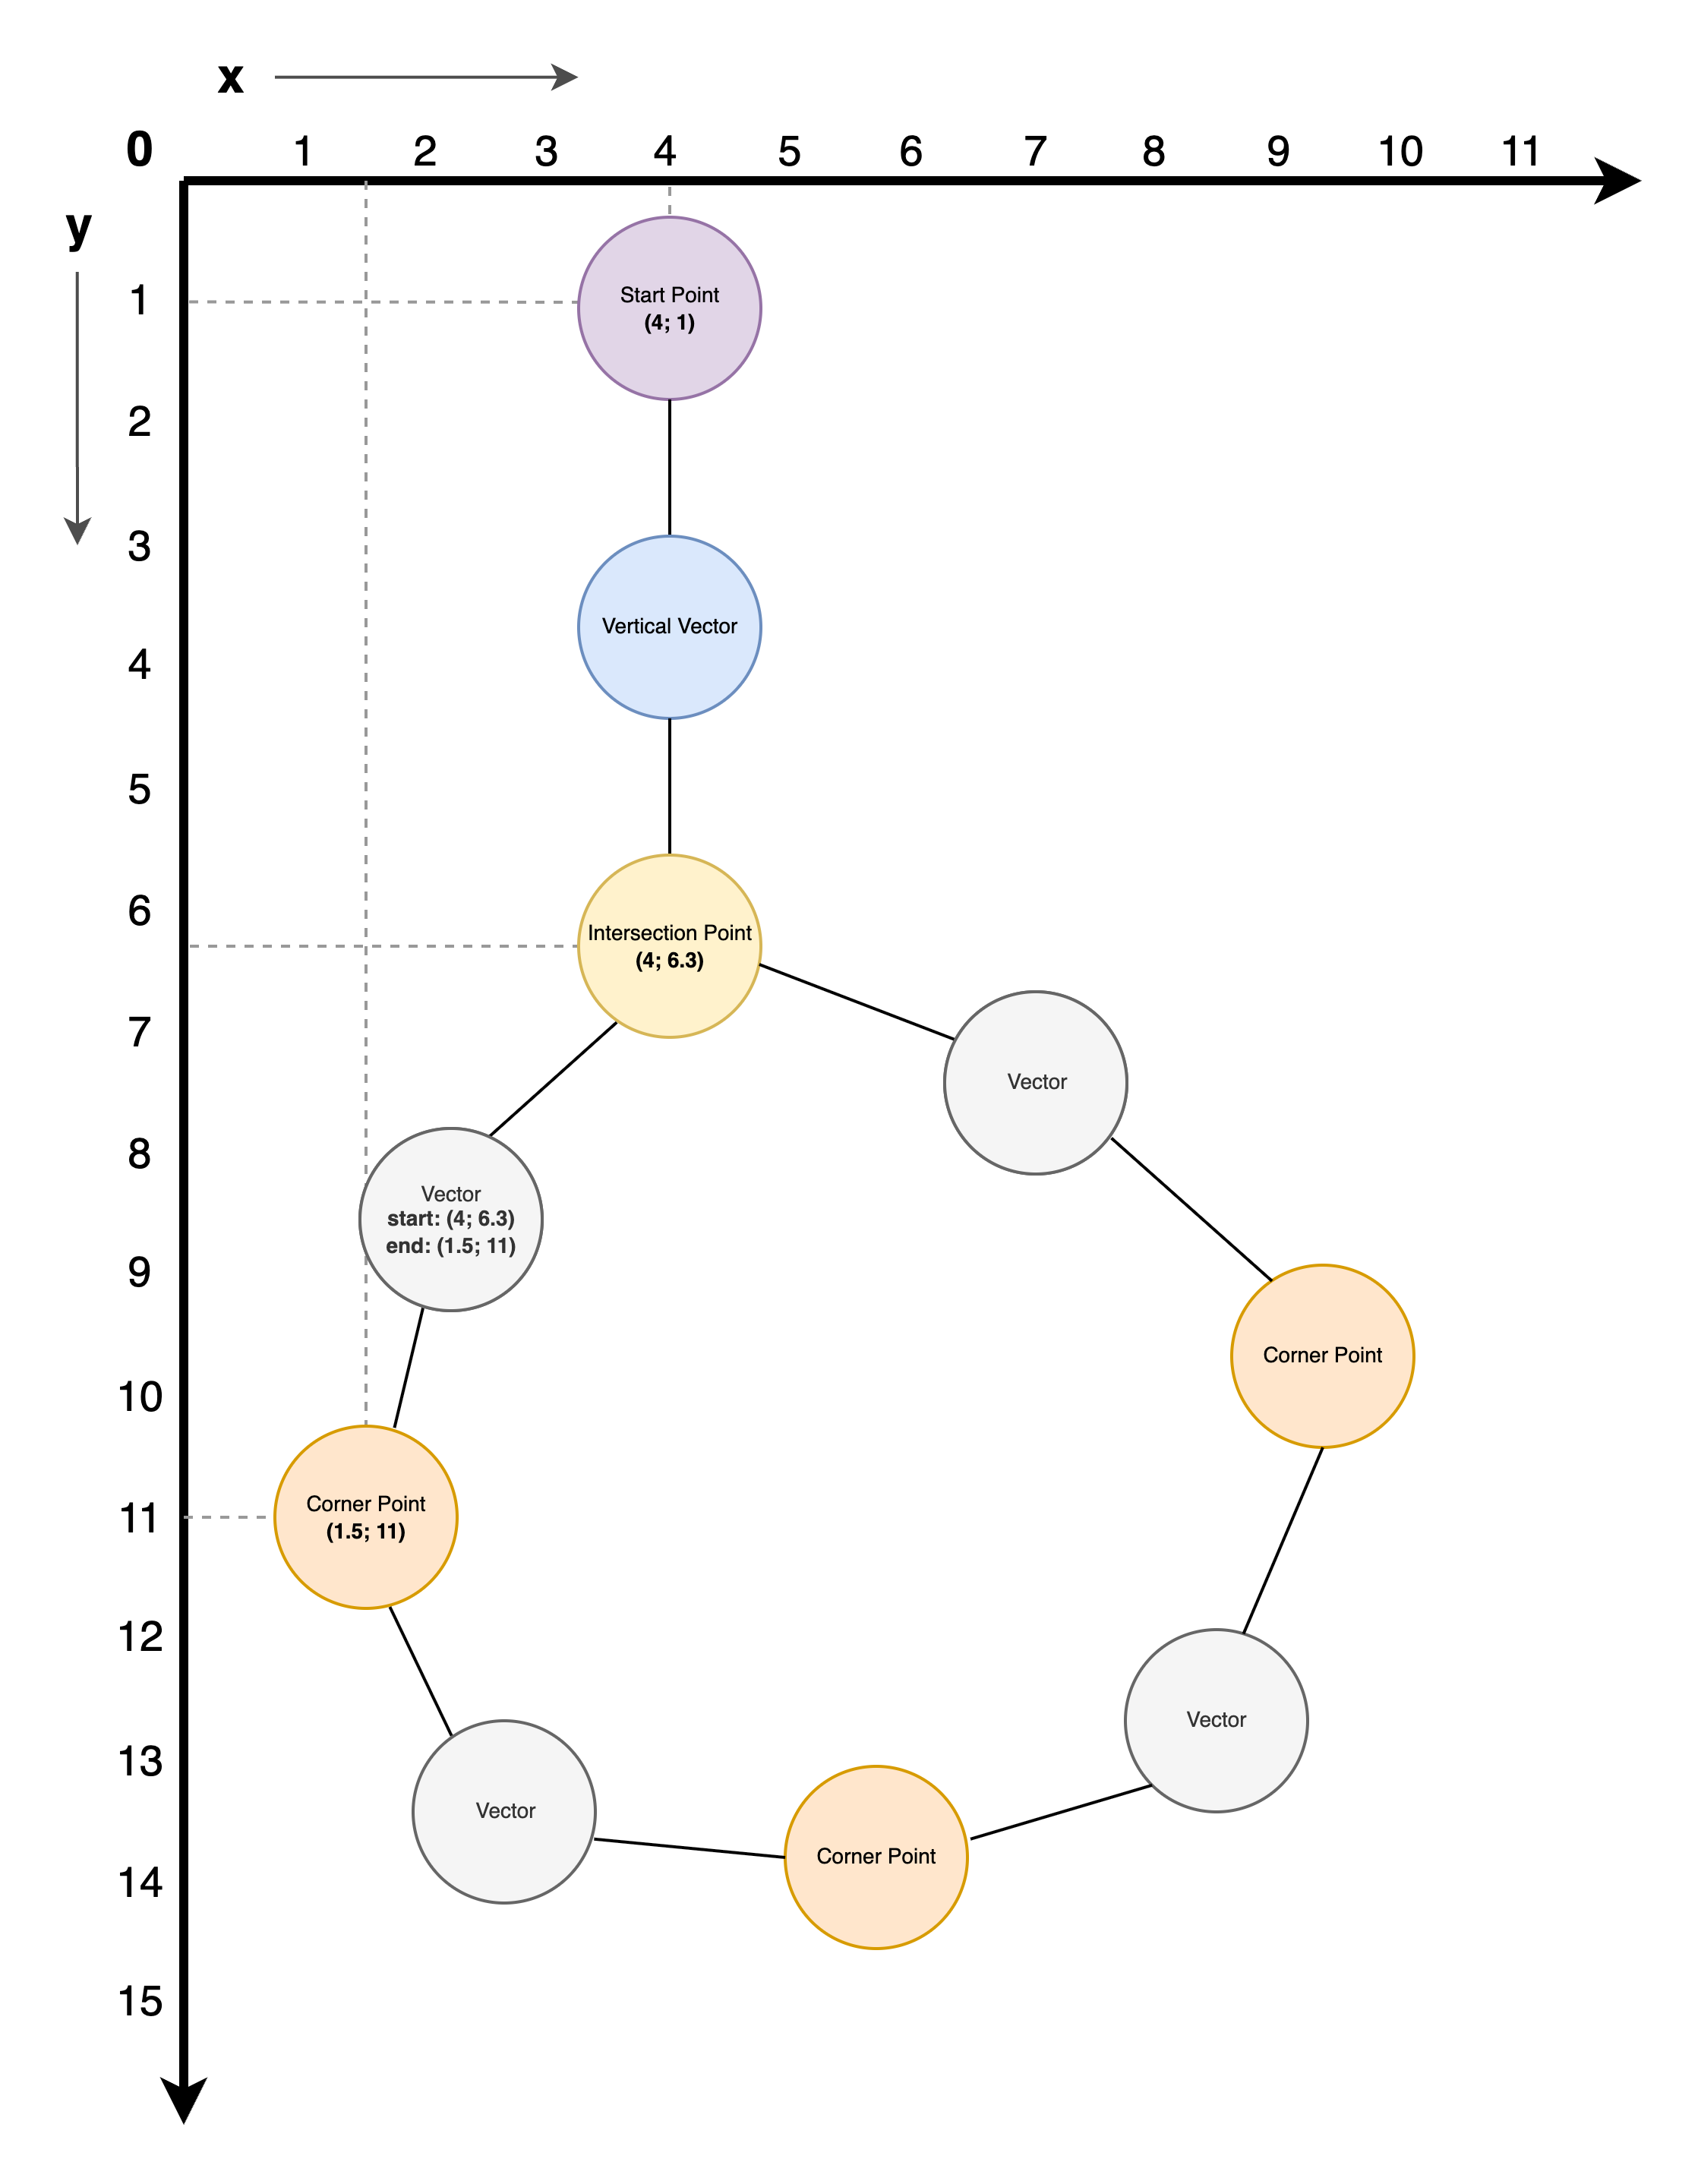
\includegraphics[width=0.45\columnwidth]{images/absolute_coordinate_system.png}
    \hfill
    
\includegraphics[width=0.45\columnwidth]{images/relative_coordinate_system.png}
    \caption{Coordinate system transformation from absolute pixel coordinates (left) with origin at top-left to normalized centered coordinates (right) ranging $[-1, 1]$. This transformation enables scale and translation invariance for concept formation.}
    \label{fig:coordinate_systems}
\end{figure}

\section{Concept Formation via Structural Reduction}

\subsection{From Multiple Graphs to Single Attractor}

Concept formation proceeds through iterative structural composition. Given training samples \(G_1, G_2, \ldots, G_n\), the algorithm initializes the concept with the first graph (\(C_0 = G_1\)) and iteratively refines it through custom reduction operations (CRO): \(C_{i+1} = \text{CRO}(C_i, G_{i+1})\) for \(i = 1, 2, \ldots, n-1\). This formulation treats the first sample as a baseline that subsequent samples refine, preserving only structural elements common across all instances.

The integration process for each sample follows five coordinated steps: (1) align start points across both graphs using clustering-based selection to establish consistent traversal origins; (2) apply critical point preprocessing through iterative reduction strategies (see~\autoref{subsec:structural_reduction_rules}) to achieve structural compatibility; (3) generate synchronized traversal paths that maintain correspondence between critical points in both graphs; (4) identify common structure along matched path segments by comparing all simple paths between consecutive critical points and selecting best matches via node similarity assessment; (5) merge geometric and semantic properties using type-specific integration strategies (see~\autoref{subsec:parametric_generalization}). Each iteration produces a refined concept \(C_i\) that represents the intersection of structural patterns encountered thus far.

Figures~\ref{fig:step1}--\ref{fig:step4} illustrate this iterative reduction process across four training samples of a handwritten digit. The progression demonstrates how the algorithm systematically eliminates sample-specific variations while preserving essential structural patterns shared across all instances.

\begin{figure}[!t]
    \centering
    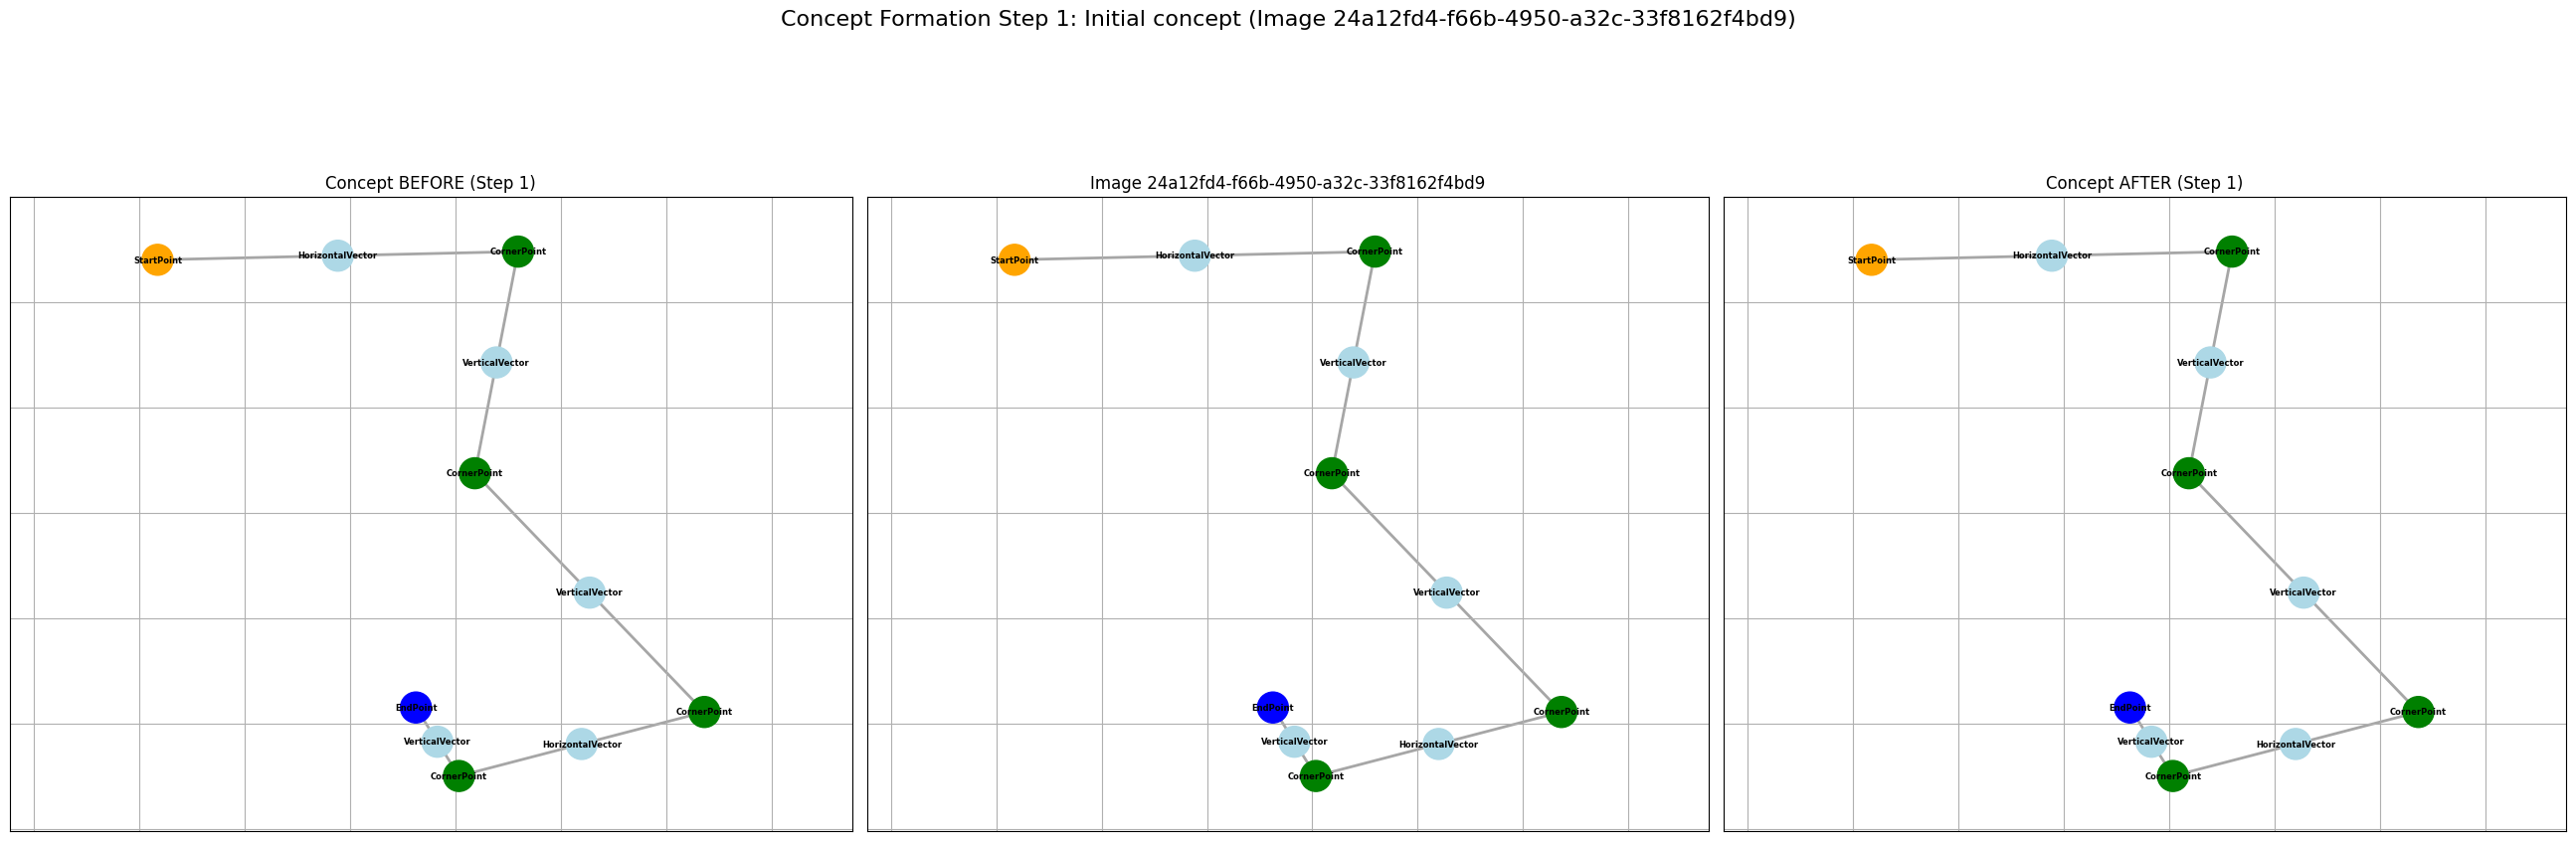
\includegraphics[width=0.9\columnwidth]{images/step_1.png}
    \caption{Step 1 (\(C_0 = G_1\)): The first training sample establishes the initial concept with complete structural detail including all endpoints, corner points, and intersection points.}
    \label{fig:step1}
\end{figure}

\begin{figure}[!t]
    \centering
    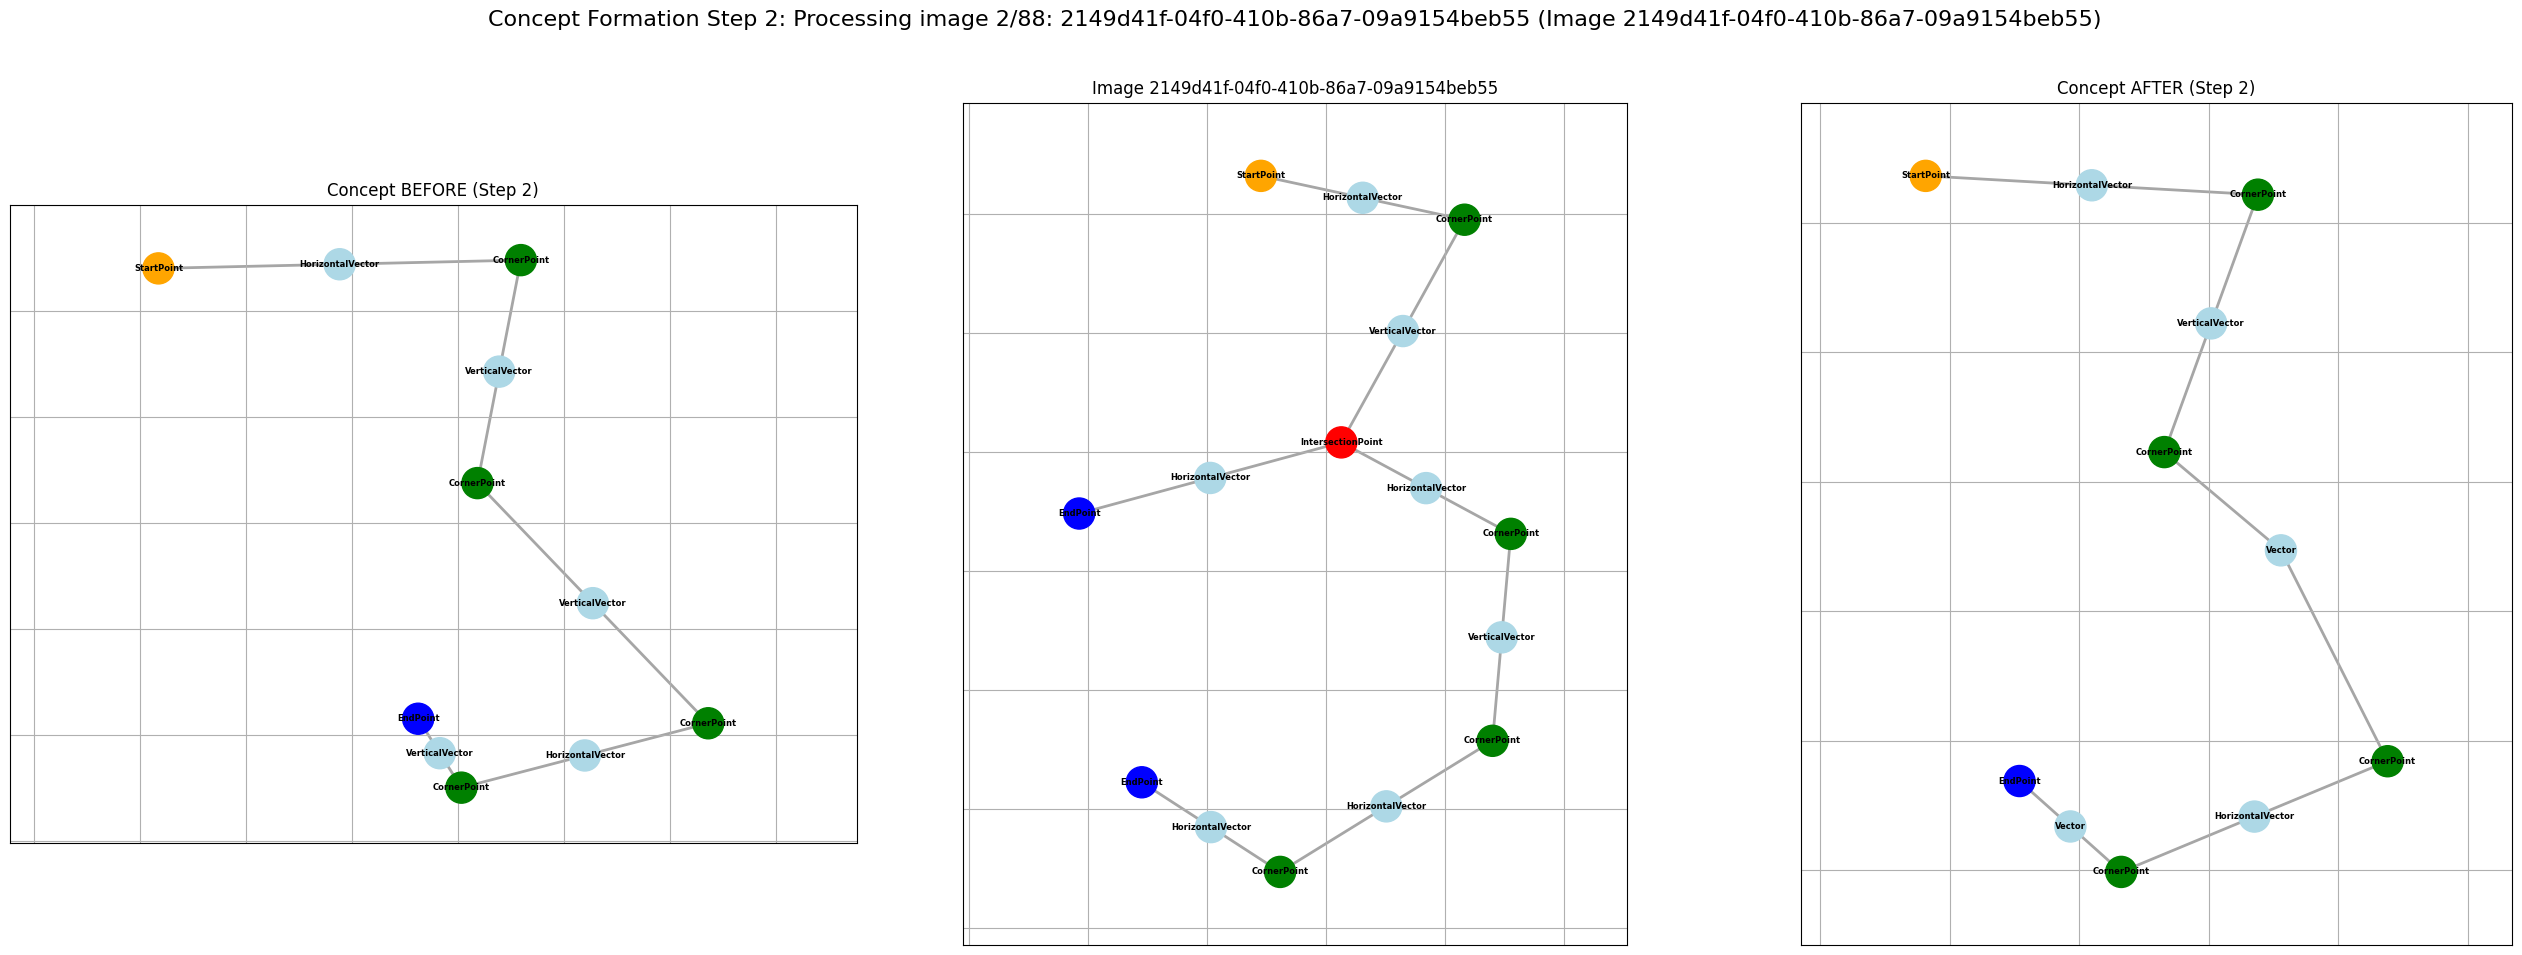
\includegraphics[width=0.9\columnwidth]{images/step_2.png}
    \caption{Step 2 (\(C_1 = \text{MCM}(C_0, G_2)\)): Integration of the second sample reveals a redundant endpoint branch. The algorithm removes the excess endpoint path and reduces the nearest IntersectionPoint to CornerPoint, then updates concept properties through parametric merging.}
    \label{fig:step2}
\end{figure}

\begin{figure}[!t]
    \centering
    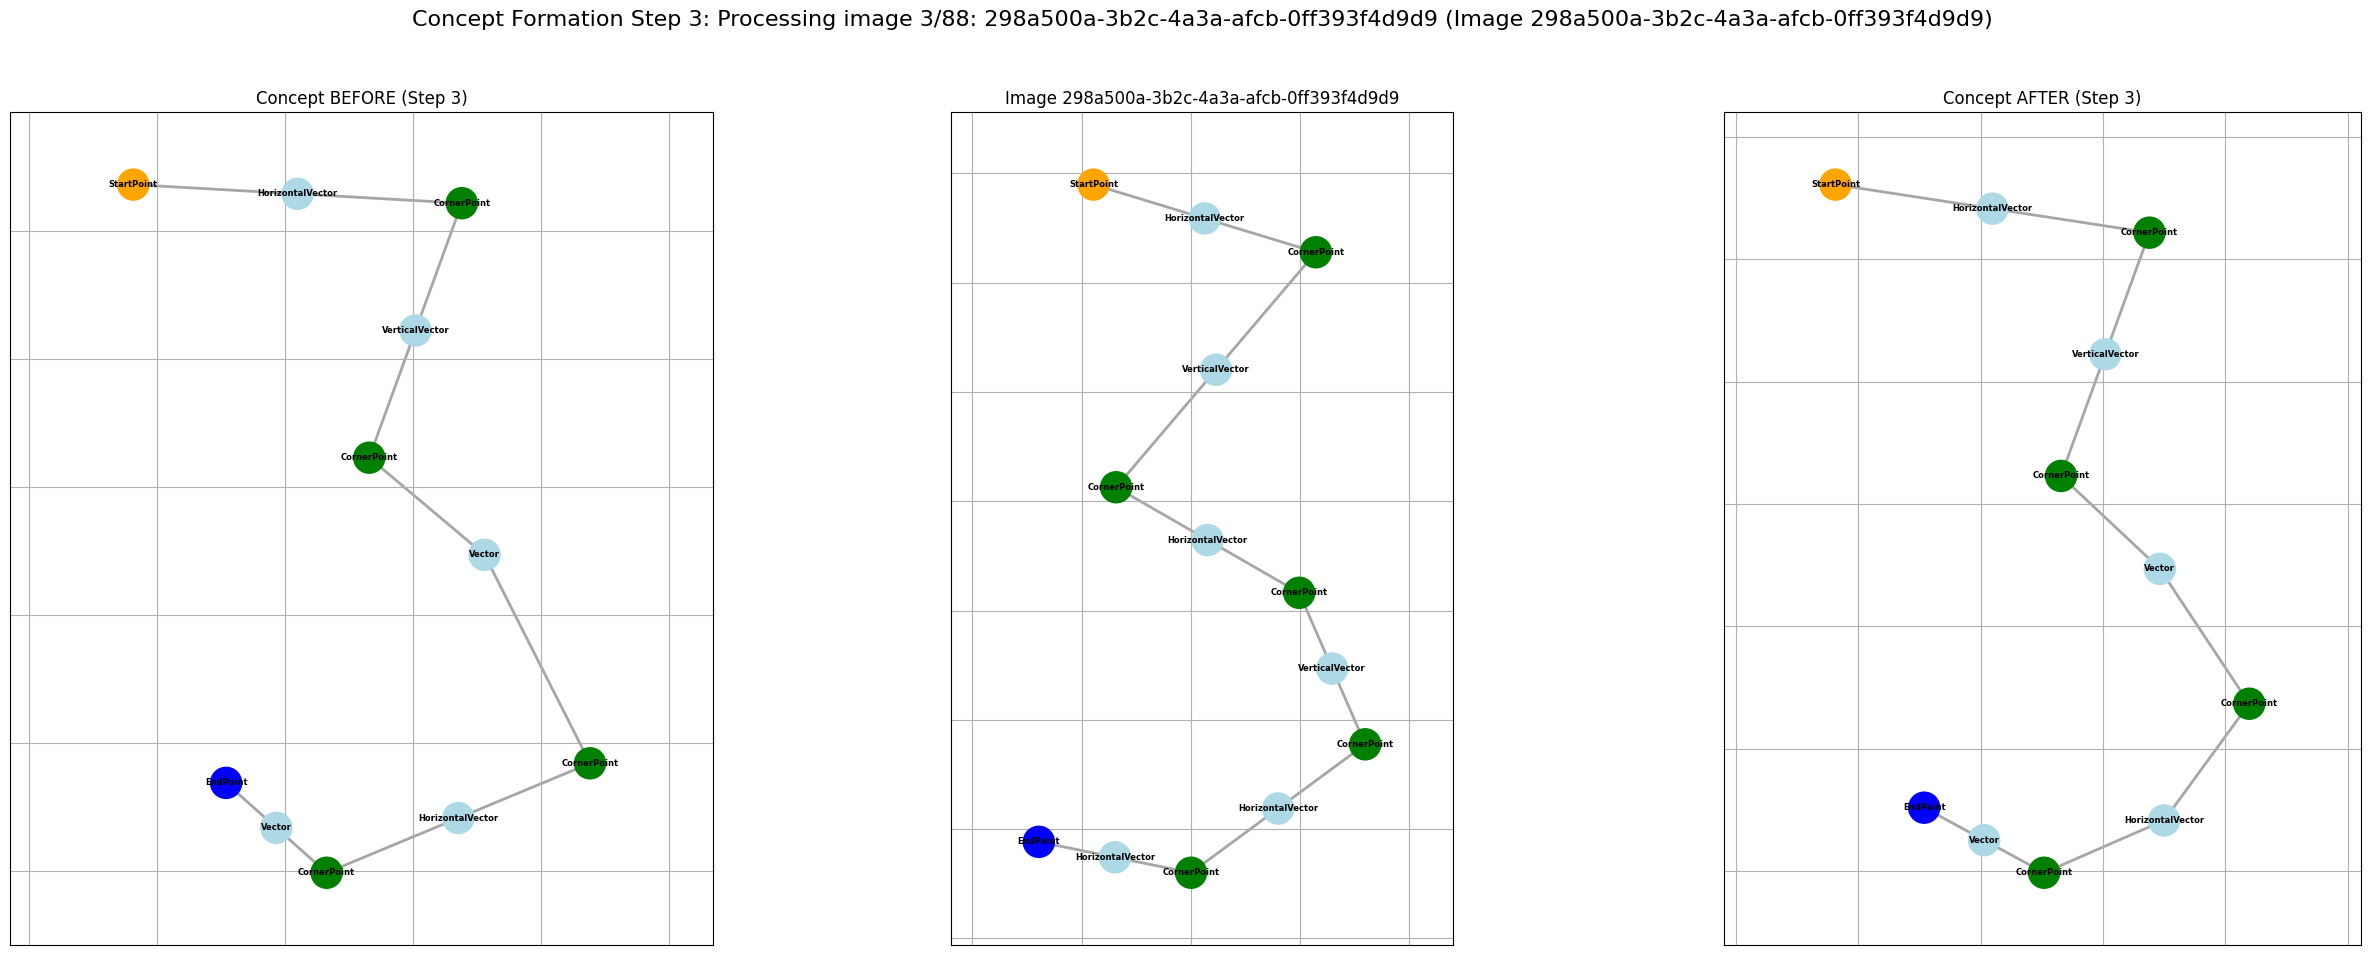
\includegraphics[width=0.9\columnwidth]{images/step_3.png}
    \caption{Step 3 (\(C_2 = \text{MCM}(C_1, G_3)\)): The third iteration identifies a redundant corner point in the lower structure. Removal and realignment of neighboring points maintains continuity while eliminating structural fragmentation. Property ranges continue to expand, capturing variation across samples.}
    \label{fig:step3}
\end{figure}

\begin{figure}[!t]
    \centering
    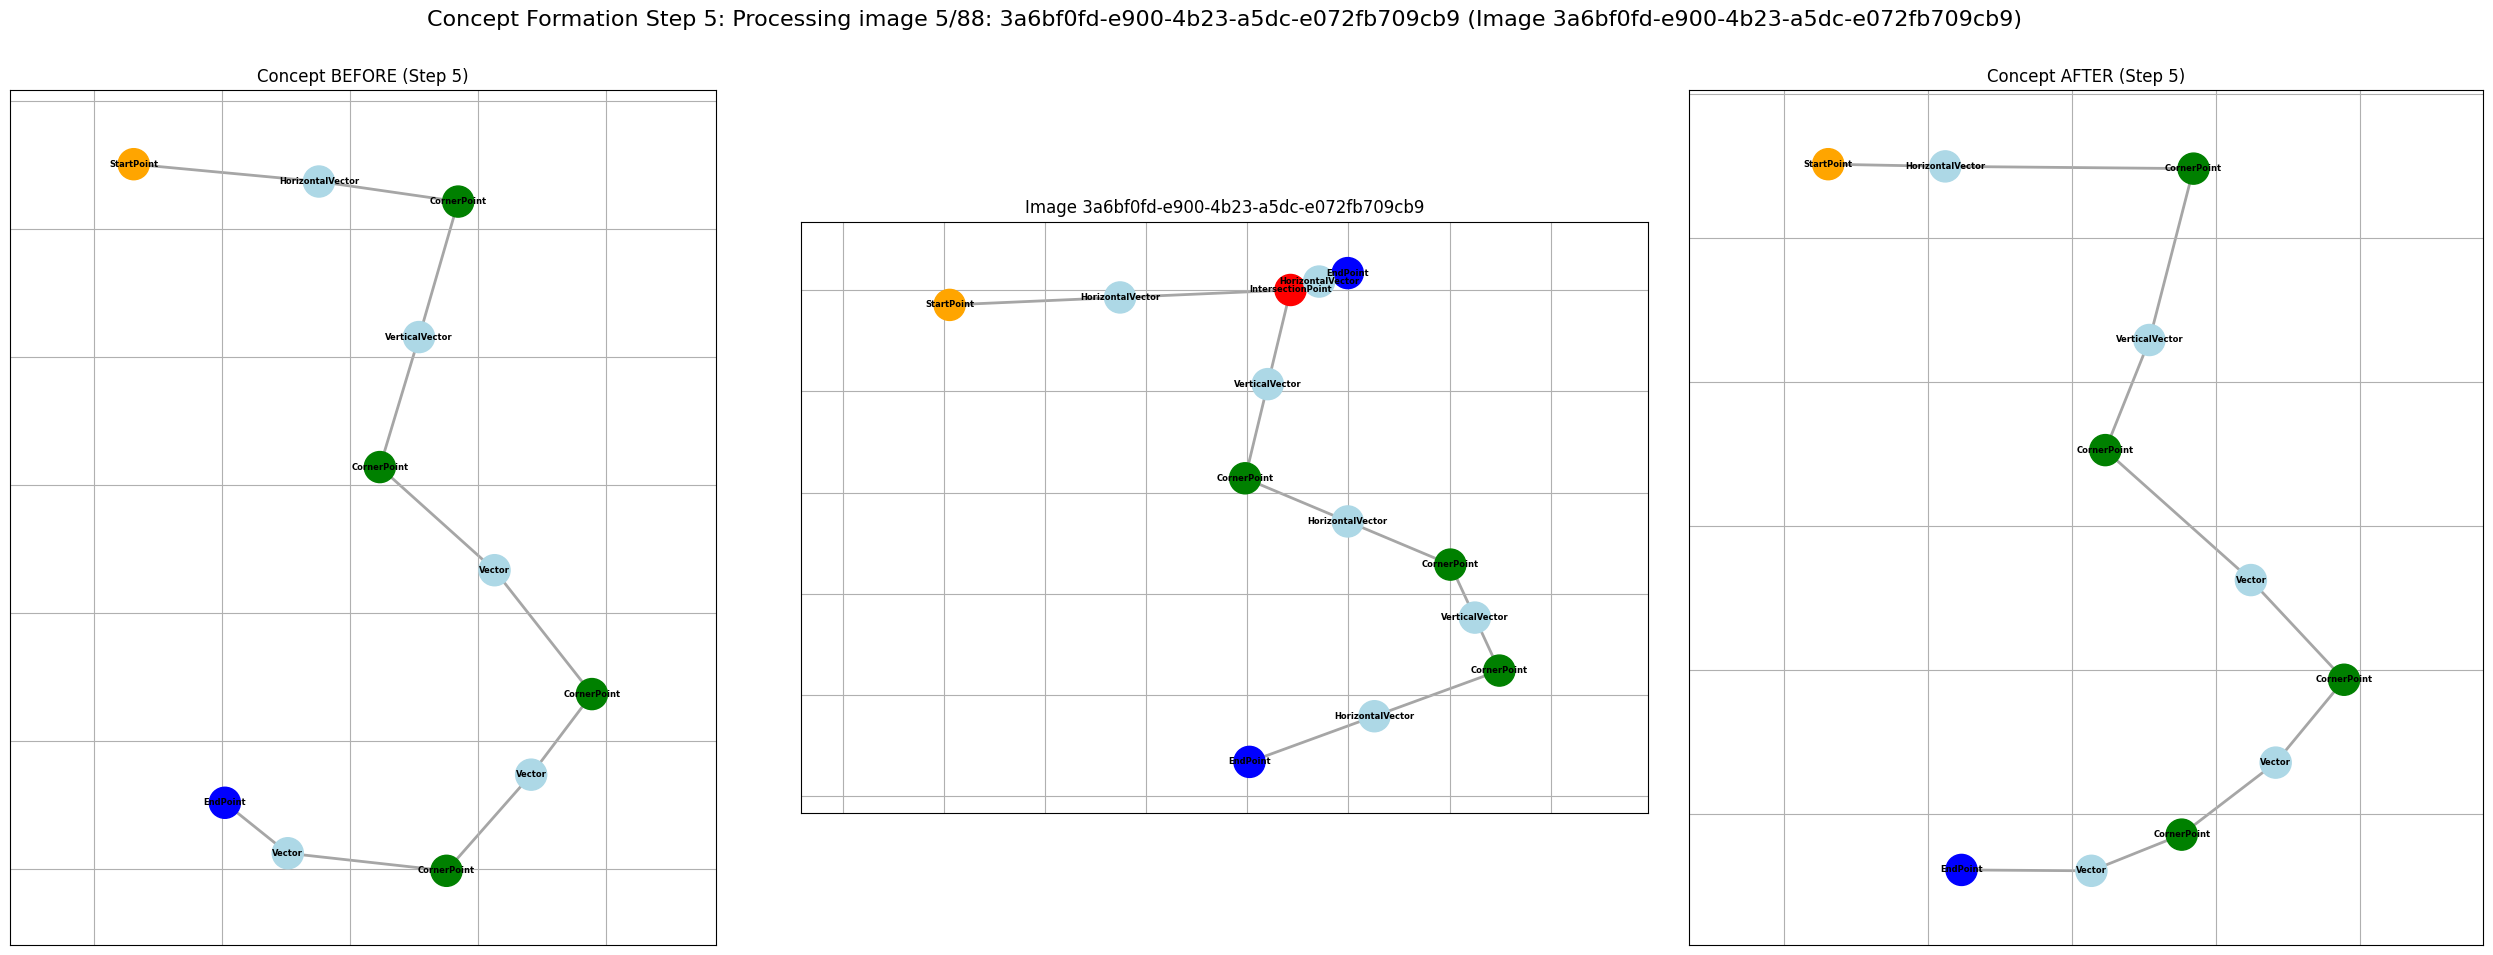
\includegraphics[width=0.9\columnwidth]{images/step_4.png}
    \caption{Step 4 (\(C_3 = \text{MCM}(C_2, G_4)\)): The fourth iteration detects noise manifested as a redundant substructure (endpoint and connecting path to nearest IntersectionPoint). Removal yields a refined concept capturing the canonical structural pattern with stabilized property distributions representing the concept attractor.}
    \label{fig:step4}
\end{figure}

\subsection{Structural Reduction Rules} \label{subsec:structural_reduction_rules}

The custom reduction operations (CRO) employs three complementary reduction strategies to align critical point structures before path-level comparison. These strategies operate within a type hierarchy where IntersectionPoint \(\to\) CornerPoint \(\to\) Point, with the constraint that StartPoint and EndPoint types cannot be reduced as they define structural boundaries.

\textbf{Endpoint removal} eliminates terminal nodes that lack correspondence across samples. The algorithm computes a similarity matrix between endpoints in the concept and image graphs, removing endpoints with maximum similarity below given threshold. When endpoint counts differ, the algorithm removes excess endpoints with the lowest maximum similarity scores. For each removed endpoint, the algorithm traverses from the terminal node toward the nearest critical point and removes the entire connecting path, eliminating sample-specific protrusions while preserving shared structural junctions.

\textbf{Intersection point merging} consolidates junction nodes representing the same structural feature. The algorithm first applies semantic reduction: any node labeled IntersectionPoint but having degree \(\leq 2\) is relabeled as CornerPoint (degree 2) or EndPoint (degree 1) to maintain type-topology consistency. When intersection counts differ between graphs, the algorithm identifies excess intersections via similarity matrix comparison (with given threshold) and removes those with lowest similarity scores. Removal proceeds by finding the path from the excess intersection to the nearest remaining critical point (preferring other intersections), removing intermediate nodes, and relinking preserved neighbors to the target junction. This operation reduces structural fragmentation while maintaining connectivity.

\textbf{Path pruning} normalizes segments between aligned critical points. For each pair of corresponding critical points, the algorithm identifies all simple paths connecting them and filters paths containing intermediate critical points to maintain segment isolation. It then computes node similarity matrices between all path pairs and selects the best matching pair based on average maximum similarity per node. Using the shorter path as a template, the algorithm matches nodes from the longer path via similarity scores and constructs the result path containing only matched positions. This template-based reduction captures essential connectivity patterns while eliminating length variations and intermediate detail specific to individual samples.

\subsection{Parametric Generalization} \label{subsec:parametric_generalization}

While structural reduction determines which nodes and edges persist in the concept graph, parametric generalization determines how their attributes are merged. The algorithm employs three distinct merging strategies based on attribute type, balancing the preservation of variation with the elimination of inconsistencies.

\textbf{Numeric properties} transform into range representations capturing central tendency and acceptable variation. For values \(v_1, v_2, \ldots, v_n\) from \(n\) training samples, the merged property becomes \(\{\text{min}: \min_i v_i, \text{max}: \max_i v_i, \text{center}: \frac{1}{n}\sum_i v_i, \text{type}: \text{``range''}\}\). This strategy applies to coordinates (\texttt{normalized\_x}, \texttt{normalized\_y}), geometric measurements (\texttt{length}, \texttt{angle}), and topological counts (\texttt{corner\_points\_count}, \texttt{intersection\_points\_count}). For example, if three samples have \texttt{corner\_points\_count} values \([5, 8, 3]\), the merged concept stores \(\{\text{min}: 3, \text{max}: 8, \text{center}: 5.33\}\), preserving both the expected value and the observed variability.

\textbf{Categorical properties} preserve only values consistent across all samples. For strings \(s_1, s_2, \ldots, s_n\), the merged property is \(s_1\) if \(s_i = s_1\) for all \(i\), otherwise the property is removed entirely. This strict matching ensures that categorical attributes in the concept represent universal characteristics rather than incidental variations. For instance, \texttt{contour\_type} values \([\text{``OPEN''}, \text{``OPEN''}, \text{``OPEN''}]\) merge to \(\text{``OPEN''}\), while inconsistent \texttt{horizontal\_direction} values \([\text{``Left''}, \text{``Right''}, \text{``Right''}]\) cause the property to be excluded from the concept.

\textbf{List properties} retain only elements present in all samples via set intersection: for lists \(L_1, L_2, \ldots, L_n\), the merged property is \(L_1 \cap L_2 \cap \cdots \cap L_n\). This strategy applies primarily to node \texttt{labels}, which encode multiple type classifications per node. For example, if three corresponding nodes have labels \([[\text{``Point''}, \text{``CornerPoint''}], [\text{``Point''}, \text{``EndPoint''}], [\text{``StartPoint''}, \text{``Point''}]]\), the merged labels become \([\text{``Point''}]\)---the sole label common to all instances. Empty intersections indicate that no universal list-based features exist for that property, and the property may be excluded or represented as an empty set depending on semantic requirements.

These merging strategies ensure that concept representations capture statistically coherent patterns: range-based merging preserves natural variation in continuous parameters, exact matching filters inconsistent categorical labels, and set intersection retains only universal structural classifications. The resulting concept graphs encode not point estimates but \emph{distributions} of acceptable values, enabling flexible matching during classification while maintaining interpretability through explicit parameter bounds.

\section{Validation on MNIST Handwritten Digits}

\subsection{Experimental Setup}
% 6 digit classes (1, 2, 3, 6, 7, 9)
% 5-6 training samples per class
% Graph extraction pipeline

\lipsum[8]

\subsection{Concept Characteristics}
% Aggregate metrics: |V|, |E|, mean degree, cycles
% Example: Digit 3 concept formation progression
% Parameter range evolution

\lipsum[9]

\subsection{Classification via Graph Matching}
% Graph Edit Distance
% Few-shot performance results

\lipsum[10]

\section{Discussion}

\subsection{Explainability Through Structure}
% Cycles → closed contours
% Node degree → branching structure
% Attribute ranges → acceptable variation
% Navigable explanations vs post-hoc attribution

\lipsum[11]

\subsection{Limitations and Future Work}
% Scalability concerns (GED complexity)
% Skeletonization dependency
% Limited rotation invariance
% Texture blindness

\lipsum[12]

\section{Conclusion}

% Brief summary of contributions:
% - Graph representation for contours
% - Concept formation through structural reduction
% - MNIST validation demonstrating viability
% - Explainability through explicit structure

\lipsum[13]

\bibliographystyle{IEEEtran}
\bibliography{references}

\end{document}

